\lab{Algorithms}{Multivariate Finite Difference Schemes}{Multivariate Numerical Derivatives}
\label{Ch:Multivariate Finite Difference Schemes}

\objective{Understand how to compute numerically the Jacobian and Hessian of a function.}

The Jacobian is a generalization of the derivative in many dimensions. We can think of it, 
intuitively, as defining a linear approximation to the function in a neighborhood of some given
point. If the function happens to be real-valued, the Jacobian defines a tangent plane to the graph of 
the function at a point. 
The Jacobian is of critical importance in a variety of areas, and we will use it in lab \ref{lab:NewtonsMethod}
to find zeros of multivariate functions.

Formally, the Jacobian of a function $f:\mathbb{R}^n \rightarrow \mathbb{R}^m$ is an $m \times n$ matrix. It is defined by the formula:
\begin{equation*}
J_{ij} = \frac{\partial f_i}{\partial x_j}
\end{equation*}

We can use finite difference approximations to find partial derivatives in the natural manner:
\begin{equation*}
\frac{\partial f}{\partial x_i} (x) \approx \frac{f(x+h e_i)-f(x)}{h}
\end{equation*}
where $e_i$ is a unit vector in the $i$th coordinate (the direction $x_i$). Higher order approximations and centered and backwards differences follow by naturally extending this definition.

\begin{problem}
Write a function \li{Jacobian} that accepts a function handle, an integer giving the dimension of the
range of the function, an integer giving the dimension of the domain of the function, a NumPy array giving
the point at which to approximate the Jacobian, and an optional argument giving the step size $h$. Use center approximation of order 1.
Return a NumPy array giving the approximated Jacobian matrix at the given point.

If the function under consideration maps from $\mathbb{R}^n$ to $\mathbb{R}^m$, the function handle should
accept as input an array of shape \li{(n,)} and return an array of shape \li{(m,)}.

Test your function on the following $f: \mathbb{R}^2 \to \mathbb{R}^2$:
\begin{equation*}
f(x, y) =
\begin{pmatrix}
e^{x} \sin(y) + y^3 \\
3y - \cos(x)
\end{pmatrix}
\end{equation*}

Compare your \li{Jacobian} function against the analytically computed derivative on the square $[-1,1] \times [-1,1]$ using ten thousand grid points (100 per side). Which method is faster? What is the maximum error of your function?
\end{problem}

Given a function from $\mathbb{R}^n \to \mathbb{R}$, sometimes the mixed partial derivatives are useful. In particular, the mixed partials will be useful when we study optimization in Volume 2. This information is contained in the Hessian matrix, which is defined as

\begin{equation*}
H_{ij} = \frac{\partial^2 f}{\partial x_i \partial x_j}
\end{equation*}

We can use the following formula to approximate mixed partial derivatives
\small
\begin{equation*}
\frac{\partial^2 f}{\partial x_i \partial x_j} = \frac{f(x + (e_i + e_j)h) - f(x + (e_i-e_j)h) -f(x + (e_j-e_i)h) + f(x - (e_i + e_j)h)}{4h^2}
\end{equation*}
\normalsize

\begin{problem}
Write a Python function that numerically calculates the Hessian of a given function. 
The function should be named \li{Hessian}, and should accept as inputs a function handle, 
an integer giving the dimension of the domain of the function, a NumPy 
array giving the point at which to approximate the Hessian, and an optional argument giving the 
step size.
Return the approximated Hessian matrix at the given point.

Test it on the following function
\begin{equation*}
f(x,y) = (1-x)^2 + 100(y-x^2)^2
\end{equation*}
This function is known as the Rosenbrock Banana function, or Rosenbrock's Valley. It is a common test function for optimization algorithms because it is non-convex and the global minimum is hard to find from certain starting points. A graph is shown in figure \ref{Fig:Rosenbrock}. Compare the output of your function with the analytic solution on the region $[-2,2] \times [0,2]$, using ten thousand points. What is the maximum error of your function?
\end{problem}
\begin{figure}
\begin{center}
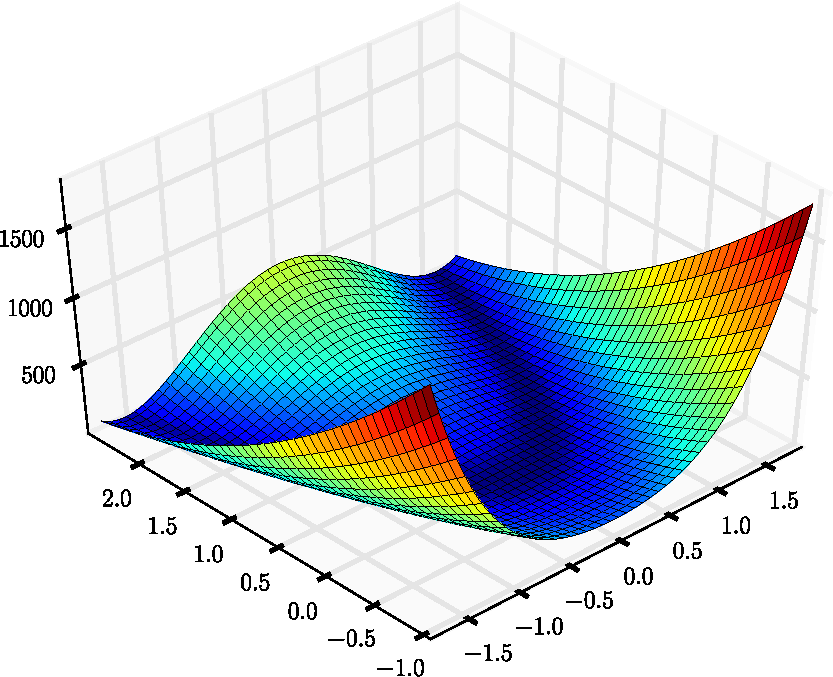
\includegraphics[width = \textwidth]{Rosenbrock}
\caption{The Rosenbrock Banana Function, a common test function in optimization algorithms}
\label{Fig:Rosenbrock}
\end{center}
\end{figure}
